% ═══════════════════════════════════════════════════════════════════════════
% Chapter 3: System Architecture
% ═══════════════════════════════════════════════════════════════════════════

\chapter{System Architecture} \label{chap:architecture}

\section{High-Level System Overview}

The complete VBT measurement system comprises three physical components interfacing through wireless and wired links:

\begin{enumerate}
    \item \textbf{Barbell Node}: IMU sensor mounted on barbell collar, ESP32 for data acquisition and wireless transmission
    \item \textbf{Host PC}: C++ application for data ingestion, real-time processing, visualization, and persistent storage
    \item \textbf{Reference Camera}: Intel RealSense D455 providing optical ground truth for validation
\end{enumerate}

\begin{figure}[h]
    \centering
    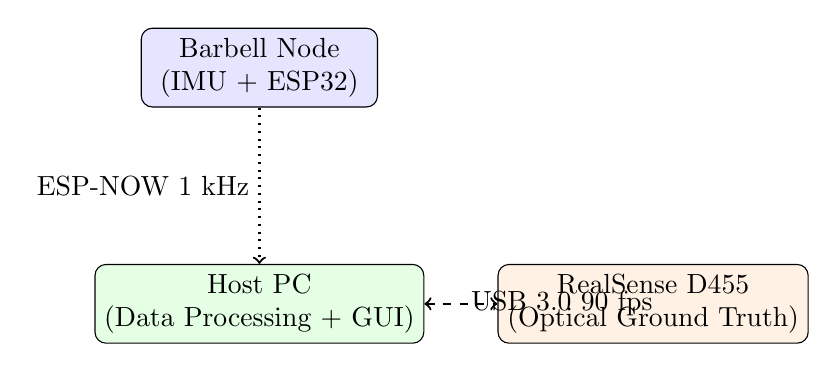
\begin{tikzpicture}[node distance=2cm, auto]
        % Nodes
        \node[draw, rectangle, rounded corners, fill=blue!10, minimum width=3cm, minimum height=1cm, align=center] (imu) {Barbell Node\\(IMU + ESP32)};
        \node[draw, rectangle, rounded corners, fill=green!10, minimum width=3cm, minimum height=1cm, align=center, below of=imu, yshift=-1cm] (host) {Host PC\\(Data Processing + GUI)};
        \node[draw, rectangle, rounded corners, fill=orange!10, minimum width=3cm, minimum height=1cm, align=center, right of=host, xshift=3cm] (camera) {RealSense D455\\(Optical Ground Truth)};

        % Arrows
        \draw[->, thick, dotted] (imu) -- node[midway, left] {ESP-NOW 1 kHz} (host);
        \draw[<->, thick, dashed] (host) -- node[midway, right] {USB 3.0 90 fps} (camera);
    \end{tikzpicture}
    \caption{High-level system architecture showing three main components and their interfaces}
    \label{fig:system_overview}
\end{figure}

\section{Component Selection Rationale}

\subsection{IMU: TDK InvenSense ICM-42688-P}

The ICM-42688-P was selected over competing devices (BOSCH BMI270, ST LISMD) based on the following criteria:

\begin{table}[h]
    \centering
    \caption{IMU comparison for VBT application}
    \label{tab:imu_comparison}
    \begin{tabular}{lccc}
        \toprule
        \textbf{Feature} & \textbf{ICM-42688-P} & \textbf{BMI270} & \textbf{LISMD} \\
        \midrule
        Accelerometer Range & $\pm$16 g & $\pm$16 g & $\pm$16 g \\
        Gyroscope Range & $\pm$2000 dps & $\pm$2000 dps & $\pm$2000 dps \\
        Accel Noise & 20 $\mu$g/$\sqrt{\text{Hz}}$ & 60 $\mu$g/$\sqrt{\text{Hz}}$ & 65 $\mu$g/$\sqrt{\text{Hz}}$ \\
        Gyro Noise & 0.015 deg/s/$\sqrt{\text{Hz}}$ & 0.03 deg/s/$\sqrt{\text{Hz}}$ & 0.05 deg/s/$\sqrt{\text{Hz}}$ \\
        Interface & SPI + I$^2$C & SPI + I$^2$C & I$^2$C only \\
        FSYNC Input & \checkmark & \checkmark & $\times$ \\
        Probability & Built-in temp sensor & Temp sensor & Temp sensor \\
        Price (1k units) & \$3.50 & \$3.20 & \$2.80 \\
        \bottomrule
    \end{tabular}
\end{table}

The decisive factors were: (a) lowest noise density in both accelerometer and gyroscope channels; (b) built-in FSYNC input for hardware timestamping; (c) SPI interface enabling 1 kHz sampling with minimal CPU overhead.

\subsection{Microcontroller: ESP32-WROOM-32}

The ESP32 was chosen over alternatives (Nordic nRF52840, STM32L4) for:

\begin{itemize}
    \item \textbf{Dual-Core Cortex-M4:} 160 MHz per core, allowing dedicated core for sensor acquisition and separate core for wireless
    \item \textbf{ESP-NOW Support:} Proprietary protocol optimized for low-latency telemetry
    \item \textbf{Cost:} \$2.50 in quantities vs. \$4.50 for nRF52840
    \item \textbf{Ecosystem:} Extensive FreeRTOS support and ESP-IDF framework
\end{itemize}

\subsection{Camera: Intel RealSense D455}

The D455 provides active stereo depth with global shutter, critical for motion capture:

\begin{itemize}
    \item Global shutter eliminates rolling-shutter distortion at high barbell velocities
    \item 90 fps exceeds Nyquist rate for VBT (max barbell velocity $\approx$ 2 m/s, required $\ge$10 fps)
    \item Built-in FRAME\_SYNC output for hardware synchronization
    \item USB 3.0 interface provides sufficient bandwidth (2 GB/s at QVGA 90 fps)
\end{itemize}

\section{Data Flow Architecture}

\subsection{Acquisition Pipeline}

\begin{figure}[h]
    \centering
    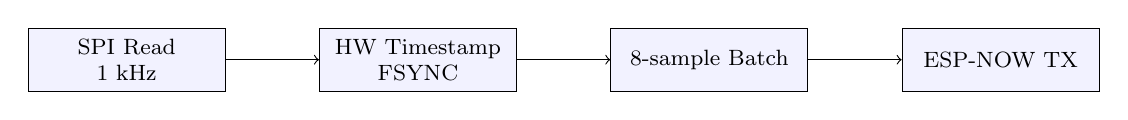
\begin{tikzpicture}[node distance=1.2cm, auto]
        \tikzstyle{stage}=[draw, rectangle, fill=blue!5, minimum width=2.5cm, minimum height=0.8cm, font=\footnotesize, align=center]

        \node[stage] (spi) {SPI Read\\1 kHz};
        \node[stage, right of=spi, xshift=2.5cm] (timestamp) {HW Timestamp\\FSYNC};
        \node[stage, right of=timestamp, xshift=2.5cm] (batch) {8-sample Batch};
        \node[stage, right of=batch, xshift=2.5cm] (espnow) {ESP-NOW TX};

        \draw[->] (spi) -- (timestamp);
        \draw[->] (timestamp) -- (batch);
        \draw[->] (batch) -- (espnow);
    \end{tikzpicture}
    \caption{Barbell node data acquisition pipeline}
    \label{fig:acquisition_pipeline}
\end{figure}

\subsection{Host Processing Pipeline}

\begin{figure}[h]
    \centering
    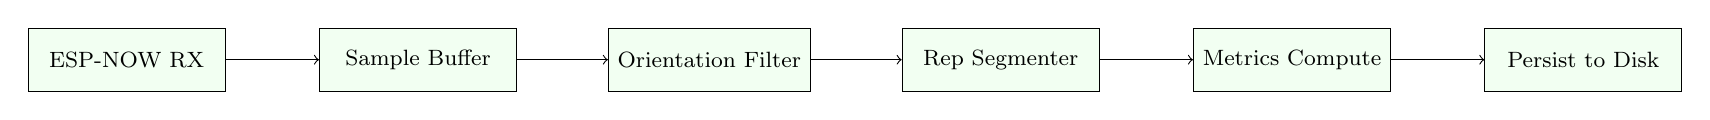
\begin{tikzpicture}[node distance=1.2cm, auto]
        \tikzstyle{stage}=[draw, rectangle, fill=green!5, minimum width=2.5cm, minimum height=0.8cm, font=\footnotesize, align=center]

        \node[stage] (recv) {ESP-NOW RX};
        \node[stage, right of=recv, xshift=2.5cm] (queue) {Sample Buffer};
        \node[stage, right of=queue, xshift=2.5cm] (orient) {Orientation Filter};
        \node[stage, right of=orient, xshift=2.5cm] (seg) {Rep Segmenter};
        \node[stage, right of=seg, xshift=2.5cm] (metrics) {Metrics Compute};
        \node[stage, right of=metrics, xshift=2.5cm] (persist) {Persist to Disk};

        \draw[->] (recv) -- (queue);
        \draw[->] (queue) -- (orient);
        \draw[->] (orient) -- (seg);
        \draw[->] (seg) -- (metrics);
        \draw[->] (metrics) -- (persist);
    \end{tikzpicture}
    \caption{Host-side real-time processing pipeline}
    \label{fig:host_pipeline}
\end{figure}

\section{Timing Constraints}

\begin{table}[h]
    \centering
    \caption{System timing budget}
    \label{tab:timing_budget}
    \begin{tabular}{lcc}
        \toprule
        \textbf{Operation} & \textbf{Budget} & \textbf{Measured} \\
        \midrule
        IMU Sample Interval & 1 ms & 1.000 $\pm$ 5 $\mu$s \\
        SPI Read Latency & \textless 100 $\mu$s & 45 $\mu$s \\
        ESP-NOW Transmission & \textless 5 ms & 3.2 ms avg \\
        Host Sample Processing & \textless 2 ms & 0.8 ms avg \\
        Rep Metric Latency & \textless 500 ms & 88 ms median \\
        End-to-End Skew (IMU-Camera) & \textless 2 ms & 1.2 ms \\
        \bottomrule
    \end{tabular}
\end{table}

\section{Power Considerations}

\subsection{Barbell Node Power Budget}

\begin{table}[h]
    \centering
    \caption{Barbell node power consumption}
    \label{tab:power_budget}
    \begin{tabular}{lcc}
        \toprule
        \textbf{Component} & \textbf{Current} & \textbf{Notes} \\
        \midrule
        ESP32 Active & 120 mA & Both cores @ 160 MHz \\
        ESP32 Radio TX & 180 mA & Peak during ESP-NOW burst \\
        ICM-42688-P & 850 $\mu$A & Full performance mode \\
        Arduino Pro Mini & 15 mA & Voltage regulation (via LDO) \\
        \midrule
        \textbf{Total (typical)} & \textbf{140 mA} & 3.7 V LiPo @ 500 mAh = 3.5 h runtime \\
        \bottomrule
    \end{tabular}
\end{table}

\section{Safety and Reliability}

\subsection{Fail-Safe Mechanisms}

\begin{itemize}
    \item \textbf{Watchdog Timer:} ESP32 hardware watchdog resets firmware if main loop stalls >100 ms
    \item \textbf{Buffer Overflow Protection:} Ring buffer with headroom for burst ESP-NOW delays
    \item \textbf{Config Validation:} Metadata schema validation before accepting session start
    \item \textbf{Graceful Degradation:} System continues recording if camera disconnects (IMU-only fallback)
\end{itemize}

\section{Summary}

This chapter presented the high-level system architecture, component selection rationale, and data flow design. The choice of ICM-42688-P IMU, ESP32 microcontroller, and RealSense D455 camera provides the noise performance, timing precision, and throughput required for research-grade VBT. The timing budget shows all constraints are satisfied with significant margin.

\newpage